% ------------------------------------------------------------------------------
% TYPO3 Version 9.4 - What's New (Italian Version)
%
% @license	Creative Commons BY-NC-SA 3.0
% @link		https://typo3.org/help/documentation/whats-new/
% @language	Italian
% ------------------------------------------------------------------------------

\section{Backend User Interface}
\begin{frame}[fragile]
	\frametitle{Backend User Interface}

	\begin{center}\huge{Chapter 1:}\end{center}
	\begin{center}\huge{\color{typo3darkgrey}\textbf{Backend User Interface}}\end{center}

\end{frame}

% ------------------------------------------------------------------------------
% Admin Panel (1)

\begin{frame}[fragile]
	\frametitle{Backend User Interface}
	\framesubtitle{Admin Panel (1)}

    The Admin Panel received a complete overhaul regarding its design as well as
    the underlying code and architecture.
	\newline\newline
	The Admin Panel is displayed at the bottom of a page in the frontend of TYPO3.
	The toggle button at the right allows integrators and editors to enable and
	disable the Admin Panel. The current state shows the \textit{enabled} state.

	\begin{figure}
		
\includegraphics[width=0.90\linewidth]{BackendUserInterface/AdminPanelEnabled.png}
	\end{figure}

\end{frame}

% ------------------------------------------------------------------------------
% Admin Panel (2)

\begin{frame}[fragile]
	\frametitle{Backend User Interface}
	\framesubtitle{Admin Panel (2)}

	Example screenshot below shows TypoScript options.

	\begin{figure}
		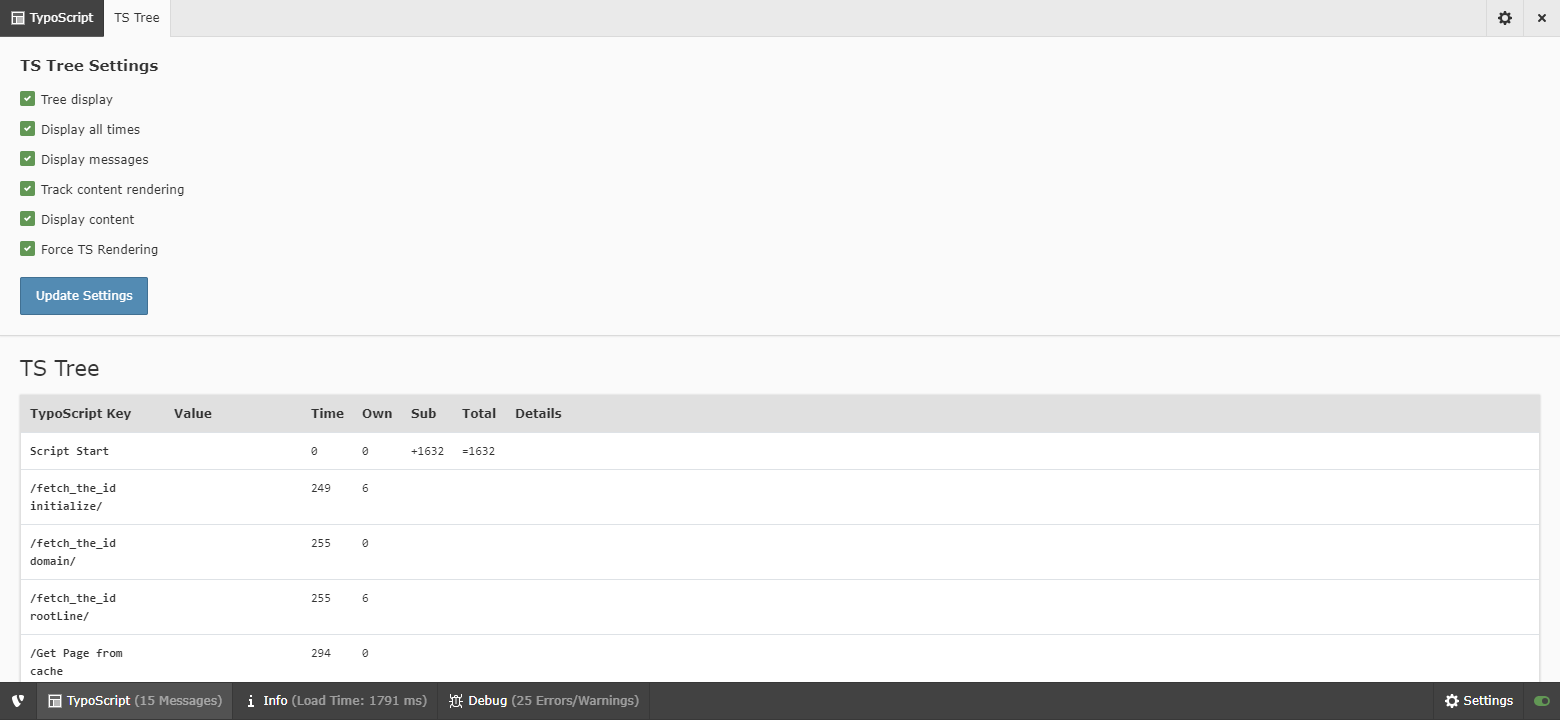
\includegraphics[width=0.90\linewidth]{BackendUserInterface/AdminPanelTypoScript.png}
	\end{figure}

\end{frame}

% ------------------------------------------------------------------------------
% Admin Panel (3)

\begin{frame}[fragile]
	\frametitle{Backend User Interface}
	\framesubtitle{Admin Panel (3)}

	Example screenshot below shows configuration options ("Settings").

	\begin{figure}
		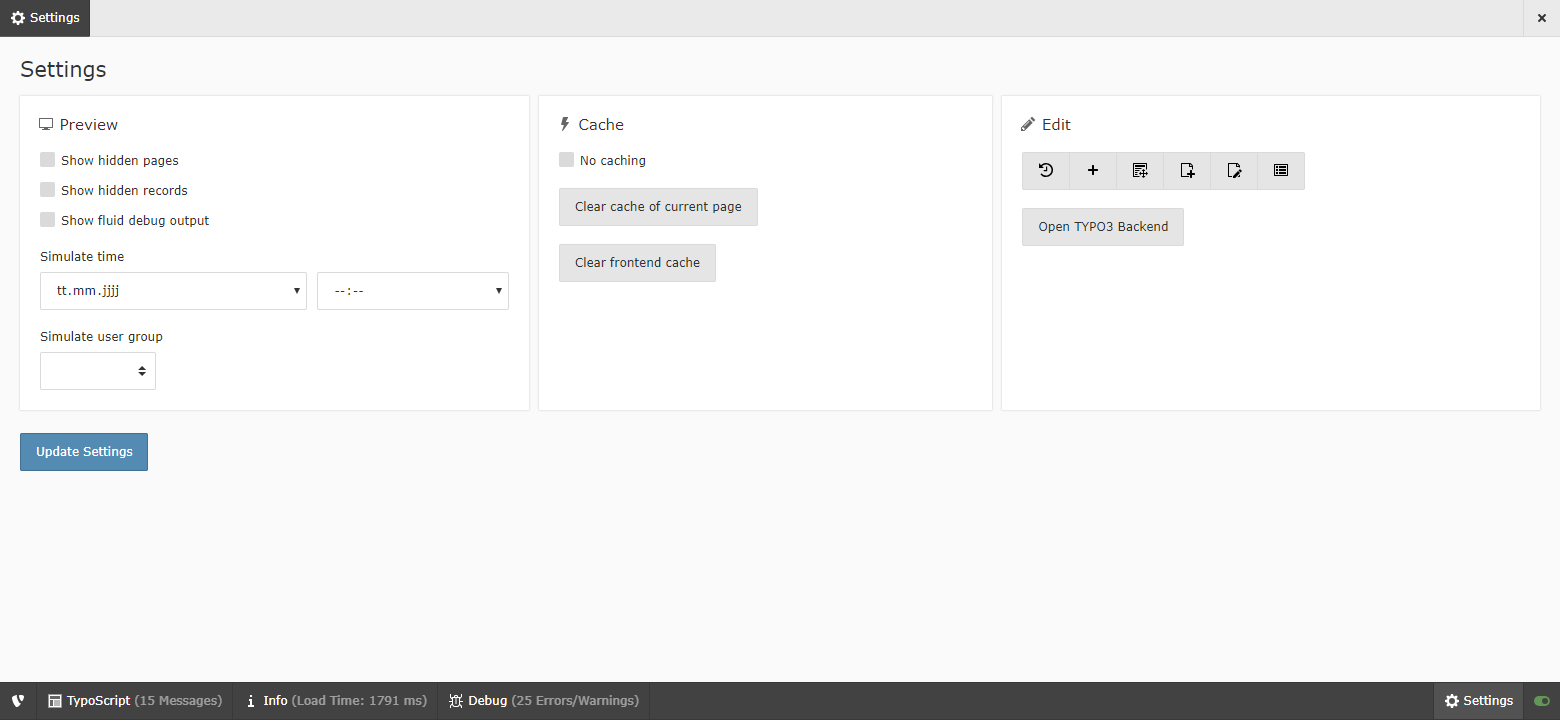
\includegraphics[width=0.90\linewidth]{BackendUserInterface/AdminPanelSettings.png}
	\end{figure}

\end{frame}

% ------------------------------------------------------------------------------
% #85398 - EXT:documentation removed

\begin{frame}[fragile]
	\frametitle{Backend User Interface}
	\framesubtitle{Extension "Documentation" Removed}

	"Documentation" module has been removed from the TYPO3 backend.
    The module had technical and conceptual flaws and acceptance within the
    community was not very high.
    \newline
    All documentation remain available at \href{https://docs.typo3.org}{docs.typo3.org}.

	\begin{figure}
		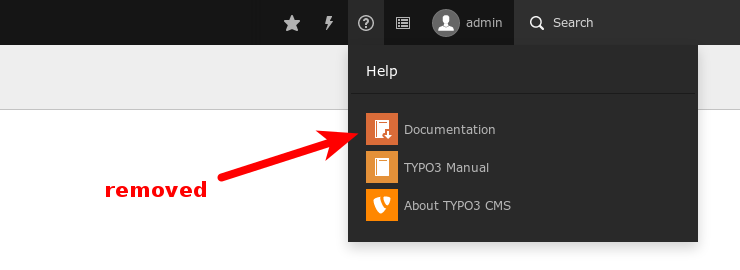
\includegraphics[width=0.70\linewidth]{BackendUserInterface/85398-ExtensionDocumentationRemoved.png}
	\end{figure}

\end{frame}

% ------------------------------------------------------------------------------
% #13265 - Select first element of page tree toolbar on initialization

\begin{frame}[fragile]
	\frametitle{Backend User Interface}
	\framesubtitle{Page Tree toolbar}

	First element of the page tree toolbar is automatically selected on load now.

	\begin{figure}
		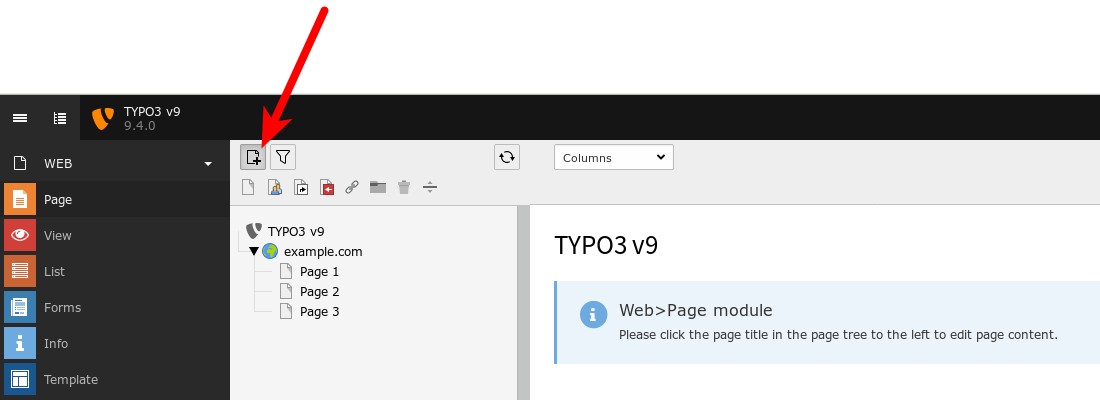
\includegraphics[width=0.90\linewidth]{BackendUserInterface/13265-FirstElementOfPageTree.png}
	\end{figure}

\end{frame}

% ------------------------------------------------------------------------------
% #85313 - Add notes field to pages table

\begin{frame}[fragile]
	\frametitle{Backend User Interface}
	\framesubtitle{Notes for Pages}

	Pages feature a "description" field (under tab "Notes") now, which allows
	users to add notes. Other backend users can see/edit these.

	\begin{figure}
		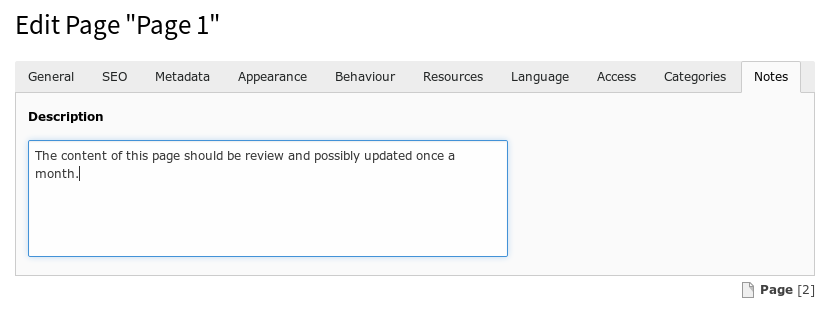
\includegraphics[width=0.90\linewidth]{BackendUserInterface/85313-NotesFieldForPages.png}
	\end{figure}

\end{frame}

% ------------------------------------------------------------------------------
% #xxxxx - Languages Visible in Frontend

\begin{frame}[fragile]
	\frametitle{Backend User Interface}
	\framesubtitle{Defined Languages Only}

	Website languages in the backend are now restricted to the languages defined
	under "Site Management → Site Configuration → Languages". Each language can
	be enabled/disabled.

	\begin{figure}
		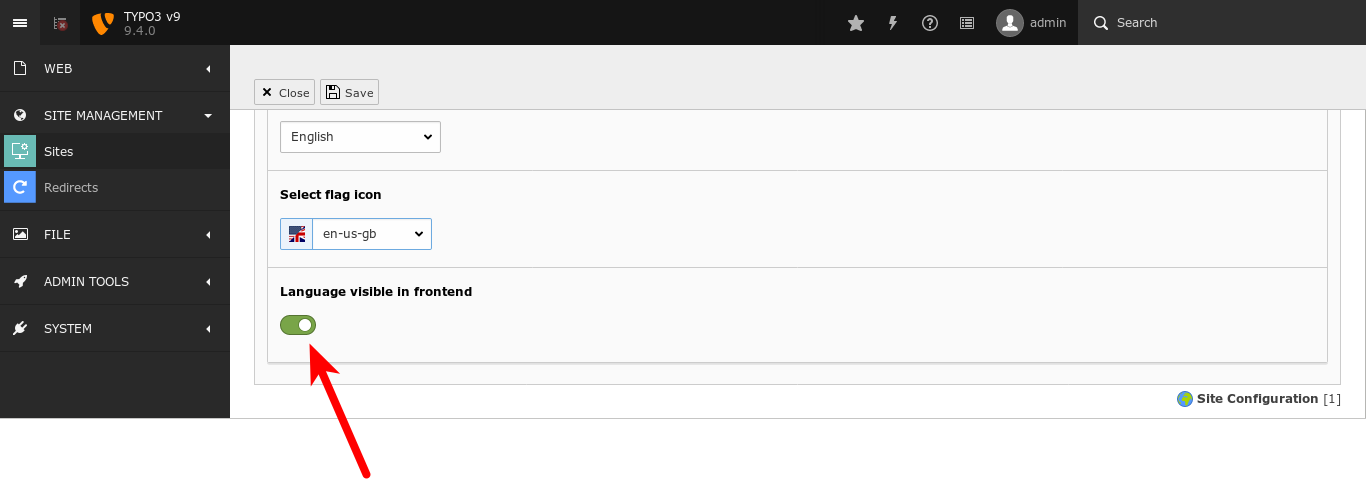
\includegraphics[width=0.90\linewidth]{BackendUserInterface/xxxxx-LanguagesVisibleInFrontend.png}
	\end{figure}

\end{frame}

% ------------------------------------------------------------------------------
% #85691 - Show page path in record info

\begin{frame}[fragile]
	\frametitle{Backend User Interface}
	\framesubtitle{Page Path in Record Info}

	Details about the reference of records now include the path in the pagetree.

	\begin{figure}
		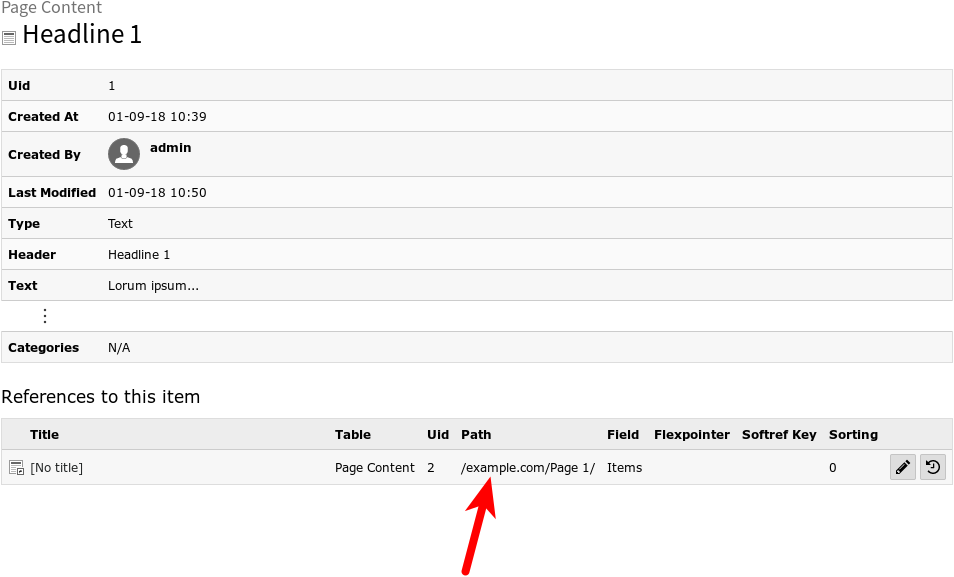
\includegraphics[width=0.70\linewidth]{BackendUserInterface/85691-ShowPagePathInRecordInfo.png}
	\end{figure}

\end{frame}

% ------------------------------------------------------------------------------
% Page-based URL Handling (aka "URL Routing")

\begin{frame}[fragile]
	\frametitle{Changes for Integrators}
	\framesubtitle{Page-based URL Handling}

 	TYPO3 supports page-based URL handling out-of-the-box now.

	\begin{figure}
		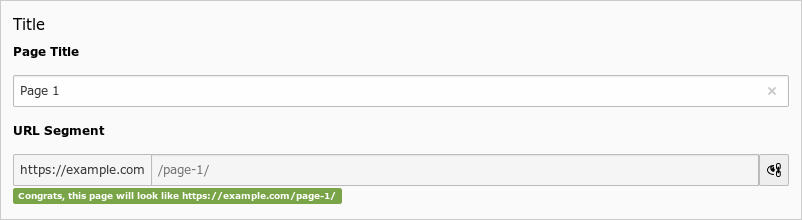
\includegraphics[width=0.90\linewidth]{BackendUserInterface/xxxxx-UrlRouting.png}
	\end{figure}

\end{frame}

% ------------------------------------------------------------------------------
% Modal Windows

% %%%%%%%%%%%%%%%%%%%%%%%%%%%%%%%%%%%%%%%%%%%%%%%%%%%%%%%%%%%%%% %
% Let's do not mention this in v9.4, but in v9.5 (TYPO3 v9 LTS). %
% We aim to achieve that all(!) popups use modal windows by the  %
% release of v9 LTS.                                             %
% %%%%%%%%%%%%%%%%%%%%%%%%%%%%%%%%%%%%%%%%%%%%%%%%%%%%%%%%%%%%%% %

%\begin{frame}[fragile]
%	\frametitle{Backend User Interface}
%	\framesubtitle{Modal Windows}
%
%	Almost all popup windows in the backend of TYPO3 are now "modal windows"
%	rather than small browser windows, which open.
%
%\end{frame}

% ------------------------------------------------------------------------------
